\section{The Garden of Allah}

\begin{quotex}
A man who fears to acknowledge his god, is unwise to set foot in the desert. The Arabs have a saying, Madame, the desert is the Garden of Allah. \flright{from \emph{The Garden of Allah}}

\end{quotex}
The desert has often had a peculiar fascination for the West. This is reflected in the movies about the Maghreb during the colonial era. (Obviously it is different now.) It's a little side hobby of mine to watch such films. Here are two of them.

\paragraph{Legend of the Lost}
\begin{quotex}
\textbf{Joe}: I can't recite any Psalms for ya'. but I know about people who believe in God. Our friend didn't! He put his faith in his father. A man! A human being! That's an easy faith to lose. I know about that, too.

\textbf{Dita}: But he was a good man. He tried to do good. He dreamed of goodness all his life.

\textbf{Joe}: I'm gettin' a little sick of this ``Poor Paul," ``Kind man," ``Full of grace." What does it take to wake you up? He didn't believe in anything but being a big-shot with God as a front. I've seen these do-gooders before; usually doin' the most good for themselves! Believing in God is different than drooling over rubies and emeralds.

\end{quotex}

\begin{wrapfigure}{rt}{.3\textwidth}
 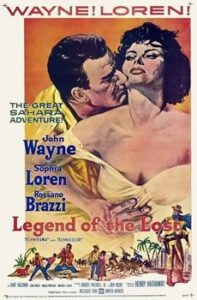
\includegraphics[scale=.5]{a20220905TheGardenofAllah-img001.jpg}
\end{wrapfigure} 

\emph{Legend of the Lost} starred \textbf{John Wayne} as Joe January, the tough guy desert guide with a soft heart that was usually kept hidden. \textbf{Sophia Loren} was Dita, the street-wise woman always seeking ways to achieve respectability. \textbf{Rossano Brazzi} played Paul, an idealist who was searching for a lost treasure discovered by his father; Paul intended to use it to help humanity. Although filmed near Tripoli, the setting Timbuktu, administered by the French at that time.

Paul had letters from his dead father that revealed the location of a treasure trove in a lost city. Paul hires Joe to guide him to it. Dita invited herself along. After a challenging journey, they found the ruins. There were three dead bodies and a diary indicating adultery and murder. Paul was devastated even after finding the gold and jewels. In the middle of the night. Paul takes the donkeys and supplies, leaving Joe and Dita without resources.

Joe, the realist, could see right through Paul's idealism. Joe is a believer and survived the desert. Paul lost his faith and was consumed by it. In many of Wayne's movies, he is saved in the end by the calvary. In this one, he and Dita are saved in a similar way, by a fortuitously passing caravan of Tuaregs.

We are not sure if Joe and Dita were meant for each other, but it seems that way.

\textbf{Moral of the Story}: Do not place your faith in men nor in their schemes.

\paragraph{The Garden of Allah}

Marlene Dietrich called John Wayne the most boring man she'd met. So it is only fair to watch Marlene in her own Maghreb film, \emph{The Garden of Allah}. Although set in the Maghreb, it was actually filmed mostly in Arizona; but is that not also Allah's Garden?

\begin{wrapfigure}{rt}{.3\textwidth}
 
\includegraphics[scale=.5]{a20220905TheGardenofAllah-img002.jpg}
\end{wrapfigure}

Domini, played by Dietrich, raised in a convent, is spiritually and emotionally lost. She said to herself, ``No one but God and I know what is in my heart." Alone in the world, even when among people, she returns to the convent and got advice from the Mother Superior who told Marlene to go to the desert because,

\begin{quotex}
``There in the solitude, you may find yourself. In the face of the infinite, your grief will vanish and you will realize that life is larger, fuller than you think."

\end{quotex}
Meanwhile, Charles Boyer played the Trappist monk Boris, who mysteriously fled from the monastery after having taken his final vows. It was doubly upsetting because only he knew the secret of making the famous liqueur that was the monastery's source of income.

When Domini went to the desert, Destiny took over when she crossed paths with Boris, now disguised as a layman. Of course, they fell madly in love with each other. Finally, she could tell him,

\begin{quotex}
``Now you also know what is in my heart."

\end{quotex}
Yet, Boris was conflicted, and his faith was endangered in the desert. Eventually, he was exposed by a French officer who had seen him at the monastery.

In those days, it was still shocking when a man rejected his final vows, unlike nowadays, when it is a matter of indifference. Domini was more understanding, although she knew that he would have to return to the monastery. She accompanies him there and when they painfully parted, she promised him,

\begin{quotex}
``We are believers, Boris, we know this isn't all, it can't be. Surely in that other world, the real and lasting world, we'll be together forever."

\end{quotex}
In the depths of her heart, Domini understood the multiple states of being. The pain of separation in this impermanent world paled in the knowledge that they would be reborn to be together forever.



\flrightit{Posted on 2022-09-05 by Cologero }
